\chapter{Preliminares}

En esta sección se presenta el marco teórico de este trabajo, dando un panorama
general de cada una de las disciplinas abordadas e introduciendo los conceptos
básicos y fundamentales para entender el proyecto. Se comienza con la definición
de la taxonomía del campo de estudio, luego \todo{describir las siguientes
secciones}

\section{Taxonomía del Campo de Estudio}

\begin{figure}
   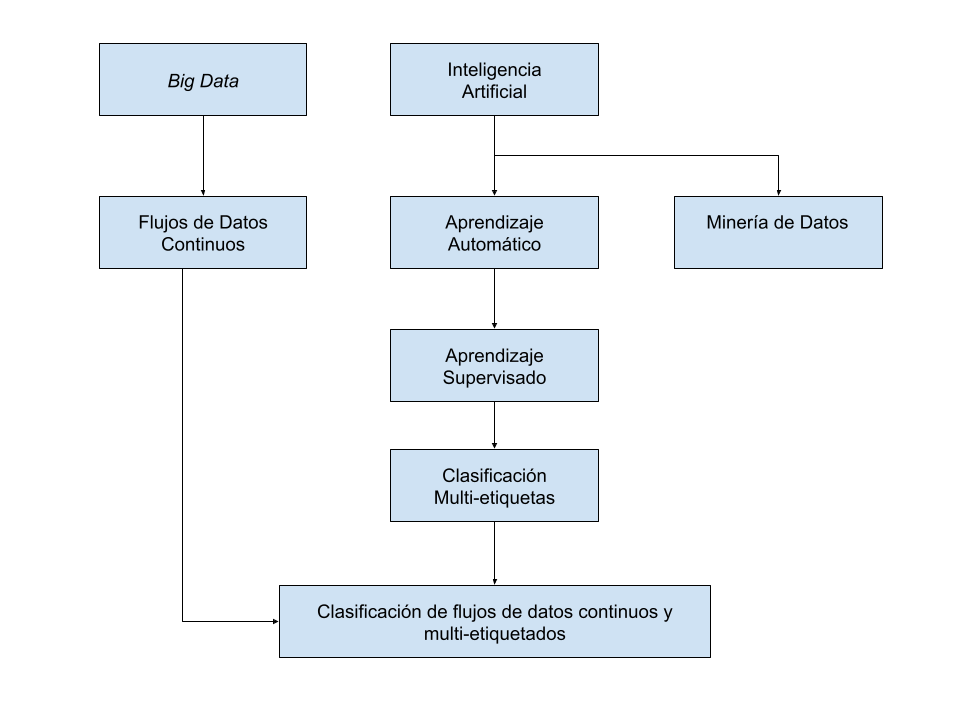
\includegraphics[width=.9\linewidth]{figures/study_field_taxonomy_v2.png}
   \centering
   \caption{Taxonomía del campo de estudio.}
   \label{fig:campo_estudio}
\end{figure}

En pocas palabras, el presente trabajo de investigación se enmarca en las áreas
de \textit{big data} y minería de datos, con aplicación en escenarios de
\textit{streaming} o flujos continuos de datos y abordando clasificaciones
multi-etiquetas. También se aprovechan técnicas del área de procesamiento de
lenguaje natural para tratar corpus de texto libre y extraer \textit{features} o
características representativas de los datos.

La figura \ref{fig:campo_estudio} es un esquema que ilustra la taxonomía del
campo de estudio y la interrelación entre las áreas de investigación
involucradas.

\section{Aprendizaje Automático}

El aprendizaje automático, también conocido por su término en ingles
\comillas{\textit{Machine Learning}}, se enmarca dentro del área de la
\acrfull{ia} y estudia cómo las computadoras pueden \comillas{aprender} o
mejorar su rendimiento meramente a partir de datos y sin la intervención de un
ser humano.  La idea detrás de esta disciplina es lograr reconocer patrones
subyacentes en los datos y tomar decisiones en base a estos. Por ejemplo, un
problema de aprendizaje automático es el de reconocer dígitos escritos a mano a
partir de un conjunto de ejemplos (ver figura \ref{fig:reconocimiento_digitos}).
Aquí se tienen un conjunto de imágenes, cada una representando un dígito del 0
al 9, y el objetivo es construir un modelo que sea capaz de detectar de qué
dígito se trata. Otro ejemplo es el de hallar documentos de texto que son
relevantes a una consulta del usuario. En este caso el modelo recibe un conjunto
acotado de términos, los cuales describen una necesidad de información del
usuario, y el modelo debe ser capaz de retornar los documentos que satisfacen la
consulta.  

Estos problemas se suelen categorizar en aprendizaje supervisado o no
supervisado, de acuerdo a si se conoce o no de antemano el concepto o etiqueta
que define a los datos. Se desarrollará más sobre este punto en las próximas
secciones. De entre los problemas de aprendizaje supervisado se destaca aquí el
de clasificación, el cual será descrito a continuación.

\begin{figure}
   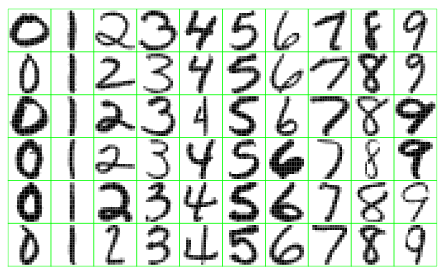
\includegraphics[width=0.66\linewidth]{figures/digits_recognition_v2.png}
   \centering
   \caption{Dígitos escritos a mano. Fuente: \citetitle{hastie_elements_2009}
   (\citeyear{hastie_elements_2009}).}
   \label{fig:reconocimiento_digitos}
\end{figure}

\section{Clasificación}

\subsection{Definición}
\label{clasificacion}

La clasificación es una tarea de minería de datos muy popular que consiste en
hallar modelos que describen la o las clases intrínsecas de los datos. La clase
corresponde a un concepto que representa al dato y es una etiqueta categórica,
es decir, un valor discreto de entre un conjunto de valores previamente
conocidos. Estos modelos, también llamados clasificadores, son capaces de
predecir la clase a la que corresponden datos previamente desconocidos. Por
ejemplo, se puede construir un modelo de clasificación para categorizar nuevos
correos electrónicos  de acuerdo a si se trata de correo basura (también
conocido como \comillas{\textit{spam}}) o no. Dicho análisis puede ayudar a
obtener un mayor entendimiento de los datos a alto nivel. Las tareas de
clasificación han sido aplicadas en áreas tales como las de aprendizaje
automático, reconocimiento de patrones o estadística. En un principio, buena
parte de los algoritmos se ejecutaban en memoria, con la limitación de espacio
de almacenamiento que eso conlleva. Investigaciones más recientes han
desarrollado técnicas para escalar los algoritmos de tal manera que puedan
manejar datos de mayor tamaño, alojados en memoria, en disco o procesados bajo
demanda. Las aplicaciones para este tipo de tareas son numerosas y entre ellas
se encuentran las de detectar fraudes o realizar diagnósticos médicos, entre
otras.

La clasificación de datos consta de dos etapas, una de aprendizaje y otra de
clasificación o predicción. Durante la tarea de aprendizaje se construye el
modelo de clasificación  el cual describe un determinado número de clases o
conceptos. También se conoce esta etapa como la de entrenamiento ya que se
selecciona un subconjunto de los datos, llamado conjunto de entrenamiento, que
consta de instancias o tuplas seleccionadas aleatoriamente y con una o más
etiquetas asociadas. Formalmente, el problema de clasificación puede ser
formulado de la siguiente manera. Se recibe un conjunto etiquetado de
instancias, tupas o ejemplos de la forma $( X, y )$ donde cada tupla es un
vector $X=(x_{1},x_{2},\dots,x_{n})$, siendo cada valor una característica
distintiva, atributo o \textit{feature} de la instancia. El vector $y$ por su parte toma
un valor de entre $n$ clases diferentes.

Este tipo de tareas se engloban dentro del campo de aprendizaje supervisado ya
que para cada instancia la etiqueta es conocida de antemano, y es aprovechada
para guiar o, siguiendo la metáfora, \comillas{supervisar} el aprendizaje del
clasificador. Esta es la diferencia principal contra algoritmos de aprendizaje
no supervisado, en los cuales la etiqueta no es conocida y se deben aplicar
técnicas para salvar esta restricción.

La primera etapa de una clasificación puede ser vista también como el
aprendizaje de una función $y=f(X)$ que pueda predecir la clase $y$ para una
tupla $X$. Por ejemplo, $X$ podría ser un mensaje de correo y la etiqueta $y$ la
decisión de si se trata de un correo basura o no. Desde esta perspectiva
queremos aprender una función que sea capaz de distinguir las clases
subyacentes.  Usualmente, esta asociación es llevada a cabo por algoritmos de
aprendizaje, los cuales internamente usan funciones matemáticas o reglas de
decisión. Algunos ejemplos de este tipo de algoritmos son los árboles de
decisión, \textit{naive} bayes, perceptrón, entre otros.

En la segunda etapa el modelo es usado para clasificar. En primer lugar, se
calcula una métrica de evaluación, tal como la exactitud o \textit{accuracy}.
Durante la etapa de entrenamiento esta estimación puede ser imprecisa, tomando
un valor que tiende a ser \comillas{optimista} o que da un valor de exactitud
mayor al rendimiento real. Esto sucede porque el clasificador puede llegar a
incorporar anomalías particulares en el conjunto de datos de entrenamiento. Este
fenómeno es llamado sobreajuste u \comillas{\textit{overfit}} y una técnica para
reducirlo es separar de entre los datos un subconjunto de prueba o de
\textit{testing} que no se usa durante el entrenamiento y a partir del cual se
realizan predicciones y se calculan las métricas de evaluación. En este
contexto, la tarea de evaluación es fundamental ya que es la vía a partir de la
cual se determina qué algoritmos o técnicas son más apropiados que otros para un
problema en particular. Además provee la información necesaria para corregir o
ajustar los parámetros de los algoritmos y así obtener modelos más robustos.

En definitiva, ambos pasos se aplican consecutivamente con el objetivo de lograr
hallar un modelo capaz de predecir etiquetas en instancias nuevas y
desconocidas.

\subsection{Algoritmos}
\label{clasificacion_algoritmos}

Como se mencionó en la sección anterior, una de las etapas de clasificación
consiste en generar un modelo capaz de clasificar instancias desconocidas. En
esta etapa se pueden aplicar diversos tipos de algoritmos de acuerdo a la
naturaleza de la tarea en particular que se desea abordar. A continuación se
describen algunos algoritmos para generar modelos y que son particularmente
relevantes para este trabajo de investigación.

\subsubsection{\textit{Naive} Bayes}

\textit{Naive} Bayes es un modelo de clasificación computacionalmente simple
pero cuyo rendimiento es competitivo contra otros modelos más complejos. Se dice
que es un clasificador estadístico ya que se basa en el teorema de Bayes. La
idea es computar una probabilidad para cada una de las clases, basada en los
atributos de la instancia y seleccionar aquella de mayor probabilidad. El
término \comillas{\textit{naive}} es el inglés para el término
\comillas{\textit{ingenuo}} y nace de la presunción que hace el algoritmo de que
los atributos son independientes entre sí, o condicionalmente independientes.
Esta presunción raramente se cumple en los escenarios donde se aplica pero
contribuye a su simplicidad computacional y a su velocidad durante el
entrenamiento.

El teorema de Bayes se define formalmente de la siguiente manera:

\begin{equation}
   P(H \mid X) = \frac{P(X \mid H) P(H)}{P(X)}
\end{equation}

En esta ecuación, el vector $X$ es una tupla definida tal como en la sección
anterior y en términos bayesianos representa la \comillas{evidencia}. $P(X)$,
por lo tanto, es la probabilidad de que la tupla contenga los atributos que
posee. Por su parte, $H$ es la hipótesis de que la tupla pertenece a una
determinada clase y $P(H)$ su probabilidad. Esta es conocida como probabilidad
\comillas{a priori}. De la misma manera, $P(H|X)$ es la probabilidad de que la
hipótesis $H$ sea cierta bajo la evidencia $X$. A esta se la llama probabilidad
\comillas{a posteriori} con $H$ condicionada por $X$ y es el valor que se quiere
determinar en una tarea de clasificación.  Finalmente, $P(X|H)$ indica la
probabilidad de que la tupla tenga unos atributos determinados dado que se
satisface la hipótesis.

Por su parte, la fórmula de \textit{Naive} Bayes es similar:

\begin{equation}
   P(C_{i} \mid X) = P(X \mid C_{i}) P(C_{i})
\end{equation}

Aquí el término $P(X)$ es descartado ya que se asume constante para todas las
clases. La hipótesis $H$ es representada como $C_{i}$ que es un valor de la
tupla $C=(C_{1},C_{2},\dots,C_{m})$, donde $m$ es el número de clases. La
presunción \comillas{ingenua} es aplicada para el cálculo del término $P(X \mid
C_{i})$ gracias a lo cual se puede definir de la siguiente manera:

\begin{equation} 
   P(X \mid C_{i}) = \prod\limits_{k=1}^n{P(x_{k} \mid C_{i})} =
   P(x_{1} \mid C_{i}) \times 
   P(x_{2} \mid C_{i}) \times \dots, \times 
   P(x_{n} \mid C_{i})   
\end{equation}

Finalmente, el modelo seleccionará la clase que maximice el valor de
probabilidad.  

Como se ha dicho anteriormente, la simplicidad, velocidad computacional y su
competitividad en métricas de exactitud hacen de \textit{Naive} Bayes un
algoritmo destacado en el campo de aprendizaje automático
\cite{wickramasinghe_naive_2020} y ha sido aplicado para problemas diversos,
tales como el de hallar errores en programas de computación
\cite{arar_feature_2017}, predecir enfermedades del corazón
\cite{dulhare_prediction_2018} o detectar ataques en una red de computadoras
\cite{kalutarage_detecting_2015}.


\subsubsection{Árboles de Decisión}

Los árboles de decisión son un modelo de clasificación que se destaca por ser de
fácil interpretación e intuitivo para el ser humano. De hecho, se puede generar
una representación gráfica del árbol generado para asistir a la comprensión del
del modelo y de cómo se comporta durante una predicción. En cuanto a su
estructura, un árbol de decisión contiene nodos, cada uno representando un
atributo de la colección. Estos nodos se conectan con otros nodos a partir de
enlaces o \comillas{ramas} que representan un valor o un rango de valores de ese
atributo. Los nodos de menor jerarquía son llamados \comillas{hojas} y contienen
la clase de la predicción, y el nodo de mayor jerarquía es llamado
\comillas{raíz}. Al momento de predecir una instancia nueva, la clasificación se
realiza de la siguiente manera:  se toma la instancia nueva, la cual no tiene
una etiqueta asociada, y los valores de sus atributos son comparados contra los
del árbol, luego se traza un camino desde el nodo raíz hasta la hoja que
contiene una clase y dicha clase es la predicción resultante. 

Los árboles de decisión se generan a partir de un algoritmo de inducción.
Existen varios de estos algoritmos pero todos son variantes que han sido
diseñadas bajo un misma principio: construir  el árbol de una manera
\comillas{voraz} \footnote{Se le llama voraz o \textit{greedy} a un algoritmo
   que busca hallar la opción óptima en cada paso y, de esta manera, alcanzar la
solución general óptima para resolver un problema.  Esto lo diferencia de
algoritmos como los de \textit{backtracking}, los cuales exploran distintas
posibilidades y pueden volver al inicio en búsqueda de una mejor solución},
comenzando desde el nodo raíz (conocido como enfoque \textit{top-down}) y
eligiendo en cada paso el atributo más informativo o que maximice alguna medida
de ganancia de información. 

Algunos de estos algoritmos son:

\begin{description} 

   \item[\acrshort{id3}] Son las siglas de \textit{\acrlong{id3}} y fue
      desarrollado en 1986 por Ross Quinlan. Consiste en crear un árbol de
      múltiples vías, buscando para cada nodo el atributo categórico que lance
      la mayor ganancia de información para las clases categóricas. Los árboles
      crecen en un tamaño máximo y luego se realiza el paso de poda para mejorar
      el poder de generalización del modelo sobre datos desconocidos.

   \item[C4.5] Es la evolución del algoritmo \acrshort{id3}. La principal mejora
      con respecto a su predecesor es que elimina la restricción de que los
      atributos deban ser categóricos. Esto lo consigue particionando el valor
      continuo en rangos o en un conjunto de intervalos discretos. C4.5
      convierte el árbol entrenado en conjuntos de reglas de decisión. 

   \item[\acrshort{cart}] Son las siglas de \acrlong{cart} y es un algoritmo muy
      similar al C4.5 pero que soporta clases numéricas, lo cual permite
      resolver problemas de regresión. 

\end{description}

Una tarea fundamental en la generación de un árbol es definir un criterio de
división para seleccionar el mejor atributo en cada paso. Existen diversas
técnicas para abordarla, una de ellas es la de \comillas{Ganancia de
Información}, usada por el algoritmo \acrshort{id3}. La Ganancia de información
busca seleccionar el atributo que posee mayor variabilidad o representatividad
de los datos y se sustenta en el cálculo de la entropía o medida de desorden. La
idea de fondo es hallar el atributo que reduzca la entropía esperada. La
entropía en el conjunto de datos $D$ se calcula de la siguiente manera:

\begin{equation}
   Entropia(D) = - \sum_{i=1}^{m} p_{i}\log_{2}(p_{i})
\end{equation}

Aquí $p_{i}$ corresponde a la probabilidad de que una tupla de $D$ corresponda a
la clase $C_{i}$.  

Luego, la ganancia de información es:

\begin{equation}
   Ganancia(A) = Entropia(D) 
   - \sum_{j=1}^{v} \frac{\left\| D_{j} \right\|}{\left\| D \right\|} 
   \times Entropia(D_{j})
\end{equation}

Aquí el atributo $A$ divide al conjunto de datos en $v$ particiones, siendo $v$
los valores posibles que toma $A$. $D_{j}$ es el subconjunto de los datos cuyas
tuplas poseen el valor $v$ del atributo $A$, siendo $\left\|D_{j}\right\|$ su
cardinalidad o número de instancias del subconjunto. Al dividir este término por
la cardinalidad del conjunto de datos, se obtiene un valor que representa el
peso de la partición y es aplicado sobre la entropía esperada.

Una vez obtenidos los valores de ganancia para cada atributo, se selecciona
aquel que maximiza la ganancia y este será el criterio de separación en el nodo.

El algoritmo C4.5 introdujo una mejora en esta técnica llamada \comillas{Razón
de Ganancia}. La misma busca disminuir uno de los efectos adversos que provoca
la técnica de ganancia de información, esta es, que tiende a favorecer a
atributos con un mayor número de valores posibles. La razón de ganancia, en
primer lugar, reemplaza la fórmula $Entropia(D)$ por la siguiente:

\begin{equation}
   EntropiaRG_{A}(D) = - \sum_{j=1}^{v} \frac{\left\| D_{j} \right\|}{\left\| D \right\|} 
   \times \log_{2}(\frac{\left\| D_{j} \right\|}{\left\| D \right\|})
\end{equation}

A su vez, el nuevo cálculo de la ganancia se formula así:

\begin{equation} \label{eq:gan_c45}
   RazonGanancia(A) = \frac{Ganancia(A)}{EntropiaRG_{A}(D)} 
\end{equation}

Finalmente, el atributo de mayor razón de ganancia es seleccionado.

\todo[inline]{Aplicaciones de árboles de decisión en la literatura}

\todo[inline]{Figura de un árbol}

\todo[inline]{Subsección para sgd?, svm?, perceptrones?}

\subsubsection{Ensambles}

Los ensambles son un conjunto de clasificadores que, al ser combinados, pueden
realizar mejores predicciones que cualquiera de ellos individualmente. En pocas
palabras, el enfoque de ensambles consiste en generar $k$ clasificadores, de un
mismo tipo o no, y entrenarlos con subconjuntos de la colección de entrenamiento
original. Dada una tupla nueva, cada clasificador devuelve su propia predicción,
llamada \comillas{voto} y luego el ensamble devuelve la predicción final basada
en esos votos.

La aplicación de ensambles en problemas de clasificación nace de la
imposibilidad de generar un único modelo capaz de generalizar lo suficiente como
para lograr un rendimiento perfecto. Ante la presencia de datos ruidosos,
atípicos o erróneos los clasificadores pueden tender a clasificar mejor para un
subconjunto de datos y no tan bien para otros. Este escenario es aprovechado por
el enfoque de ensambles ya que su éxito tiene correlación con la existencia de
diversidad en la clasificación, esto es, que haya variabilidad entre los
subconjuntos de datos, modelos o hiper-parámetros, entre otros factores. A mayor
esta diversidad, los errores particulares de un ensamble se aíslan y serán
filtrados por la clasificación final. Como resultado se espera una disminución
del error total de la clasificación así como también una mayor exactitud en la
predicción, comparando contra los clasificadores base. Por otro lado, un enfoque
de ensambles abre la posibilidad de distribuir y/o paralelizar el cómputo de la
predicción, pudiendo así mejorar los tiempos de ejecución durante el
entrenamiento.

Existen distintos tipos de ensamble, de acuerdo a su construcción y
arquitectura. A continuación se describen 3 de ellos: los ensambles de tipo
\textit{bagging}, los de tipo \textit{boosting} y los de tipo \textit{stacked}. 

\begin{description} 

   \item[Bagging] Esta es una de las primeras técnicas de ensambles conocidas y
      fue introducida por
      \citeauthor{breiman_bagging_1996}\cite{breiman_bagging_1996}. La misma se
      desarrolla de la siguiente manera: dado un conjunto de entrenamiento $D$
      con $n$  tuplas, \textit{bagging} genera un número $m$ de nuevos conjuntos
      de datos de entrenamiento, cada uno con $n$ tuplas. Para esto se toman
      tuplas del conjunto original de manera aleatoria y con reemplazo, es decir
      que puede haber tuplas repetidas y otras que no están incluidas en el
      nuevo conjunto.  Luego a partir de cada conjunto nuevo, se entrena un
      clasificador $M_{i}$. Cada clasificador puede ser del mismos tipo ya que
      la diversidad está dada por los datos. En la etapa de clasificación, cada
      modelo $M_{i}$ genera una predicción que cuenta como un voto. El ensamble
      cuenta los votos y elige la clase con mayor cantidad de votos, siendo esta
      la decisión final del ensamble.


   \item[Boosting] En la técnica de \textit{boosting} se asigna un peso a cada
      tupla de entrenamiento y se generan un conjunto de clasificadores, uno
      luego del siguiente. A diferencia del método de \textit{bagging},
      \textit{boosting} trabaja siempre sobre el mismo conjunto de datos y la
      variabilidad está dada por los pesos que son asignados. El proceso es el
      siguiente: para el primer modelo de clasificación, $M_{i}$, los pesos son
      inicializados en un mismo valor para todas las tuplas. Una vez que se
      entrena este modelo, los pesos son actualizados de tal manera que el
      siguiente clasificador $M_{i} + 1$ trate de manera particular a las tuplas
      mal clasificadas por Mi, de tal manera de llegar a una clasificación
      correcta.  El clasificador final combina los votos de cada clasificador
      individual , donde el peso del voto de cada clasificador es una función de
      su exactitud. 


   \item[Stacking] Stacking es una técnica desarrollada por
      \citeauthor{wolpert_stacked_1992}\cite{wolpert_stacked_1992} y consiste en
      entrenar un nuevo clasificador de acuerdo a las predicciones realizadas
      por otros modelos, tomando la salida de estos modelos como entrada, de tal
      manera de lograr hallar una combinación que produzca una mejor predicción.
      Este tipo de ensambles puede ser visto como un conjunto de capas. La
      primera capa consta de un ensamble de clasificadores que aprenden a partir
      de los datos de entrenamiento. Esta capa no necesariamente usa
      clasificadores del mismo tipo, mismos hiper-parámetros o particiones de la
      colección iguales, quedando estos detalles a cargo de quien diseña esta
      capa. La siguiente capa es el clasificador individual, o
      meta-clasificador, que se alimenta de las salidas de los clasificadores de
      la capa inferior y realiza el aprendizaje a partir de las clases
      producidas por estas salidas y las clases reales.

\end{description}

Una de las tareas a tener en cuenta durante el entrenamiento de un ensamble es
la de combinar las salidas de cada modelo en una salida final. La estrategia más
común y simple es la de mayoría de voto, aplicada por los métodos de
\textit{bagging}, pero existen múltiples y no necesariamente un ensamble de tipo
\textit{bagging} debe aplicar esta estrategia. Por ejemplo, algunos
clasificadores pueden decidir producir una salida sólo en el caso de que más de
la mitad de ellos coincidan, o incluso ser más restrictivos y obligar a que la
coincidencia sea total. El enfoque de \textit{boosting} por su parte, pondera al
voto de acuerdo a los pesos que calcula, dando predominio a determinadas
instancias.  También se suele dar un mayor peso a determinados clasificadores
por sobre otros. Este tipo de métodos se los denomina \comillas{mayoría de voto
ponderada} y pueden llevar a un rendimiento superior.

\todo[inline]{Aplicaciones de ensambles en la literatura}

\todo[inline]{Figura de ensamble}

\subsection{Evaluación y Métricas}
\label{clasificacion_evaluacion}

Lalalalal

\section{Clasificación Multi-etiquetas}

A diferencia del aprendizaje automático tradicional, que usa datos de etiqueta
única para representar objetos del mundo real, cada instancia en el aprendizaje
multi-etiquetas representa un único objeto pero puede contener más de una
etiqueta. Por consiguiente, la tarea de clasificación consiste hallar una
función que logre asignar a cada objeto, nuevo y desconocido, el conjunto de
etiquetas que lo caracteriza.

En este apartado se da una definición formal, se detallan las características de
un conjunto de datos multi-etiquetados y se  describen algunos métodos
tradicionales de clasificación multi-etiquetas junto con sus ventajas,
desventajas, aplicaciones y motivaciones.

\subsection{Definición Formal y Métricas}
\label{mll_def_formal}

Asumiendo que $X=\mathbb{R}^{d}$ denota el espacio de instancias $d$
dimensional, y que $Y = \{y_{1}, y_{2}, \dots, y_{q}\}$ denota el espacio de
etiquetas con $q$ etiquetas posibles, la tarea de clasificación multi-etiquetas
consiste en entrenar un conjunto $D = \{(x_{i}, Y_{i}) \mid 1 \leq i \leq m\}$
para hallar una función $h$ tal que $h: X \rightarrow 2^y$. A su vez, $X_{i}$ es
un vector de atributos $d$ dimensional definido como $(x_{i1}, x_{i2}, \dots,
x_{id})$. $Y_{i}$, por su parte, es el conjunto de etiquetas asociadas a la
instancia $X_{i}$. Luego, para cada instancia desconocida $X \rightarrow X$ el
clasificador $h$ predice $h(x) \subseteq Y$ que representa el conjunto de
etiquetas hallado para $x$.

A su vez, se definen un conjunto de métricas que describen el grado de
multi-etiquetado que tiene un conjunto de datos dado, o en otras palabras, hasta
qué punto cada ejemplo posee más de una etiqueta. Algunas de ellas son: 

\begin{description}
   \item{Cardinalidad de etiquetas}: Es el promedio de etiquetas por instancia
      del conjunto de datos. Se define como: 
      \begin{equation}
      \label{eq:mll_card}
         CardE(D) = \frac{1}{m} \sum_{i=1}^{m} \left\|Y_{i}\right\|
      \end{equation}
      Por lo tanto, a mayor el valor de cardinalidad, mayor es el número de
      etiquetas de una instancia. Por ejemplo, si $CardE = 1$, entonces la
      mayoría de ejemplos tiene una única etiqueta y, por consiguiente, se puede
      decir que la colección tiene un grado bajo de multi-etiquetado.  
   \item{Densidad de etiquetas}: Es la cardinalidad de etiquetas normalizada al
      número total de etiquetas de $D$ y se define como:
      \begin{equation}
         DenE(D) = \frac{CardE(D)}{\left\|Y\right\|}
      \end{equation}
      Así pues, un valor alto de densidad significaría que cada instancia puede
      ser una buena representación de las etiquetas del conjunto. De la misma
      manera, un valor bajo suele implicar dispersión, esto es, que la mayoría
      de las instancias tienen un subconjunto acotado de las etiquetas. 
   \item{Diversidad de etiquetas}: Es el número de conjuntos de etiquetas
      unívocos que aparecen en instancias de $D$. Se define como:
      \begin{equation}
         DivE(D) = \left\|\{Y \mid \exists x: (x, Y) \in D\}\right\|
      \end{equation}
      Aquí la interpretación es que, a mayor el valor de diversidad, menor es la
      constancia con la que las etiquetas aparecen en las instancias. De manera
      similar a la cardinalidad, el valor de diversidad también puede
      normalizarse por el número de instancias del conjunto de datos: 
      \begin{equation}
         DivEProm(D) = \frac{DivE(D)}{\left\|D\right\|}
      \end{equation}
\end{description}

\subsection{Algoritmos}

Como se había anticipado en la sección \ref{intro_mll}, la tarea de aprendizaje
sobre datos multi-etiquetados puede ser encarada siguiendo dos grandes enfoques,
llamados \comillas{Transformación del Problema} y \comillas{Adaptación del
Algoritmo}. A continuación se describen ambos enfoques y algunos de sus
algoritmos más representativos.

\subsubsection{Transformación del Problema} 

Esta categoría engloba al conjunto de algoritmos que abordan el problema de
clasificación multi-etiquetas transformándolo en múltiples problemas de
clasificación de única etiqueta, lo cual permite aplicar algoritmos de
clasificación convencionales. Tres de estos métodos son particularmente
relevantes para este trabajo: \comillas{\acrfull{br}}, \comillas{\acrfull{cc}} y
\comillas{\acrfull{lp}}.

\paragraph{\acrfull{br}}

El algoritmo de Relevancia Binaria, conocido como \textit{\acrlong{br}} en la
literatura, es un enfoque que consiste en descomponer la tarea de clasificación
\acrshort{mll} en $\left\|q\right\|$ clasificadores binarios, independientes y
de etiqueta única.  A partir de esta transformación se puede seleccionar
cualquier algoritmo de clasificación como clasificador base del problema (ver
los algoritmos presentados en la sección \ref{clasificacion_algoritmos}).  Cada
clasificador binario $g_{j}$ es entrenado con todas las instancias de la
colección pero incluyendo solo la etiqueta $j$, la cual se activa o desactiva de
acuerdo a si es relevante a la instancia. Luego la predicción de una instancia
desconocida se realiza combinando las salidas de cada clasificador individual,
esto es: 

\begin{equation}
   Y = {y_{j} \mid g_{j}(x) > 0, 1 \leq j \leq q}
\end{equation}
 
Llegado el caso en que ninguno de los clasificadores retornen etiquetas activas,
el conjunto $Y$ será vacío.

Este enfoque se dice que es de primer orden (ver sección \ref{estrategias_mll})
y no tiene en cuenta la correlación o interdependencias entre etiquetas. Este es
uno de los principales inconvenientes de este algoritmo ya que, en este tipo de
problemas de \acrshort{mll}, es usual hallar que determinadas etiquetas se
activan en conjunto con mayor probabilidad. Pese a ello, \acrshort{br} es un
enfoque muy utilizado \cite{zhang_review_2014} ya que es simple de implementar,
intuitivo y computacionalmente poco costoso en comparación con algoritmos que sí
tienen en cuenta la relación entre etiquetas.  

\paragraph{\acrfull{cc}}

Las cadenas de clasificadores o \textit{\acrlong{cc}}
\cite{read_classifier_2011} es una técnica que convierte el problema de
\acrshort{mll} en una ”cadena” de problemas de clasificación binaria, tal que el
siguiente clasificador de la cadena posee las predicciones de los anteriores. En
principio, la división del conjunto de datos es similar a la que se hace en el
enfoque anterior, designando un clasificador por cada etiqueta. Durante el
entrenamiento el clasificador inicial, seleccionado aleatoriamente, usa de
entrada los atributos originales, tal como el clasificador \acrshort{br}. Luego
la salida de este clasificador es añadida al espacio de atributos como un
atributo más de cada instancia, para que posteriormente, estos atributos sean la
entrada del siguiente clasificador, el cual también es seleccionado al azar.
proceso es repetido hasta completar todos los clasificadores.  Como se ve se
produce un ”encadenamiento” de clasificadores que no es accidental y tiene como
fin conservar la dependencia entre etiquetas, ya que cada clasificador logra
capturar la correlación entre las etiquetas de los anteriores clasificadores. 

Cabe notar que en esta técnica cobra especial importancia el ordenamiento de los
clasificadores ya que este orden tiene un impacto directo sobre el resultado de
la predicción. En otras palabras, si el ordenamiento de clasificadores se
modifica, el modelo final otorgará resultados diferentes. Para salvar esta
dificultad se han propuesto modelos como el de \acrfull{ecc}. El mismo genera un
conjunto de modelos de \acrshort{cc} con distintos ordenamientos y entrenados
con diversos subconjuntos de datos, generados con reemplazo o no. Durante la
predicción, cada cadena produce un conjunto de etiquetas, que son los votos, y
la salida final será computada por un algoritmo que combine cada salida
individual.
 
\paragraph{\acrfull{lp}}

El conjunto de potencias de etiquetas o \textit{\acrlong{lp}}
\cite{tsoumakas_random_2011} es una técnica que se encarga de transformar el
problema de \acrshort{mll} en uno de clasificación multi-clase, de tal manera de
poder abordarlo con algoritmos de este tipo. La clasificación multi-clase es un
enfoque usado para tratar con ejemplos en donde la etiqueta es única pero cuenta
con más de dos clases. Un ejemplo de este tipo de problemas es el de análisis de
sentimiento de texto, en donde las clases pueden ser \comillas{positivo},
\comillas{negativo} y \comillas{neutral}. 

En \acrshort{lp} cada etiqueta indica el subconjunto de etiquetas de
la instancia. Esto es beneficioso en cuanto a que se logra preservar la
dependencia entre etiquetas. Sin embargo, el modelo tiene algunas dificultades.
En primer lugar, el espacio de clases posibles es exponencial y su cantidad de
clases puede llegar a ser de $2^{\left\|L\right\|}$ como máximo. A su vez, pueden
llegar a arribar ejemplos con una combinación de etiquetas que el modelo no
recibió durante el entrenamiento, por lo cual no logra generalizar lo suficiente
y se lo considera un modelo incompleto. A fin de sobrepasar estas complicaciones
se desarrolló la técnica de Conjuntos Podados o \acrfull{ps}. La misma consiste
en preservar para la clasificación aquellos subconjuntos de etiquetas que son
más frecuentes en la colección, y eliminar los demás. Con esto se logra
disminuir considerablemente el espacio de clases y disminuye la complejidad
computacional, tanto durante el entrenamiento como durante la predicción.

\subsubsection{Adaptación del Algoritmo}

Además del enfoque de transformación del problema, otros autores abordan la
clasificación multi-etiquetas a partir de la adaptación de algoritmos clásicos y
bien conocidos. Esta categoría engloba al conjunto de algoritmos que abordan el
problema de \acrshort{mll} mediante la modificación de algoritmos de etiqueta
única para que sean capaces de manejar la nueva naturaleza de los datos en estas
tareas. Las modificaciones que se introducen pueden variar en complejidad según
el algoritmo tratado y las características de la colección.  Se han adaptado una
diversa cantidad de algoritmos incluyendo aquellos basados en redes neuronales,
árboles, métodos probabilísticos, entre otros \cite{herrera_multilabel_2016}.
Por mencionar algunos ejemplos, \citeauthor{gargiulo_deep_2018} usan redes
neuronales profundas para clasificar documentos de texto libre y comparan su
funcionamiento variando el número de etiquetas y aprovechando su estructura
jerárquica \cite{gargiulo_deep_2018}. Asimismo,
\citeauthor{tanaka_multi-label_2015} agregan al algoritmo de \acrshort{br} la
capacidad de capturar relaciones entre etiquetas a través del uso de árboles de
decisión y lo aplican en el área de la genómica \cite{tanaka_multi-label_2015}.

En lo que confiere a ambientes de flujos continuos de datos una de las técnicas
más populares en la literatura es la de Árbol de Hoeffding o
\textit{\acrfull{ht}} \cite{domingos_mining_2002}. A diferencia de los
algoritmos convencionales de árboles de decisión, \acrlong{ht} aborda los datos
de manera incremental. Así pues, en lugar de realizar decisiones de corte de
acuerdo a los datos previamente almacenados, \acrshort{ht} espera a tener una
cantidad suficiente de instancias para realizar el corte, con un cierto grado de
confianza. Esto significa que ya no es necesario guardar todos los datos de la
colección y que mantener una serie de estadísticas es suficiente para realizar
la clasificación. Otra de las propiedades a destacar de este método es que en
teoría se puede entrenar un árbol cuyo rendimiento se aproxime al generado en un
ambiente de \textit{batch}, con la suficiente cantidad de datos
\cite{bifet_machine_2018}. 

A partir de esto, y buscando sacar provecho de las ventajas mencionadas,
\citeauthor{read_scalable_2012} decidieron adaptar este algoritmo a problemas de
multi-etiquetas y desarrollaron el algoritmo llamado Árbol de Hoeffding
Multi-etiquetado o \textit{\acrfull{mlht}} \cite{read_scalable_2012}. Esto lo
consiguen a partir de rediseñar la fórmula de ganancia de información (ver
fórmula \ref{eq:gan_c45}) de tal manera de reflejar el impacto de todas las
clases a las cuales el ejemplo no pertenece. Desde que fue introducido en el año
\citeyear{read_scalable_2012}, \acrshort{mlht} ha sido usado como modelo de
comparación en reiteradas oportunidades \cite{sousa_multi-label_2018} y es uno
de los métodos más populares para atacar problemas de \acrshort{mll} en
ambientes de flujo continuo de datos.

Otro algoritmo muy popular para abordar este tipo de problemas y basado en
árboles de decisión incrementales es el llamado \acrshort{isoup} (siglas del
inglés \textit{\acrlong{isoup}}) \cite{osojnik_multi-label_2017}. El mismo fue
desarrollado inicialmente para hacer regresión de múltiples objetivos y luego
fue adaptado a tareas de \acrshort{mll}. Una de las novedades que introduce es
el uso de un perceptrón adaptativo en las hojas del árbol, lo cual le da la
versatilidad de poder trabajar tanto con problemas de clasificación como de
regresión.

\todo[inline]{Explicación de enfoques de ensambles? (ebr, ecc, elp)}

\subsection{Evaluación y métricas}
\label{mll_evaluacion}

Lalalalala todo

\section{Clasificación de Flujos Continuos de Datos}

\subsection{Definición}

Un flujo continuo de datos o \textit{Data Stream} es un conjunto de datos
ordenados, que arriban en el tiempo y son potencialmente infinitos. Un
\textit{stream} se define como:

\begin{equation}
   S = \{s_{0}, s_{1}, \dots, s_{t}, \dots, s_{N}\}
\end{equation}

Donde $s_{t}$ es la instancia presente en el tiempo $t$ y $s_{N}$ es el
último dato avistado en el \textit{stream}. Cada instancia $d_{t}$ posee
atributos y una o más etiquetas y se define tal como en la sección
\ref{clasificacion} de tratarse de datos uni-etiquetados o como en la sección
\ref{mll_def_formal} de tratarse de datos multi-etiquetados. 

El objetivo de la tarea de clasificación en este escenario es el mismo que para
escenarios de \textit{batch}, esto es, hallar una función capaz de enlazar
instancias nuevas con sus etiquetas correspondientes, con la salvedad de que se
debe lograr bajo restricciones de tiempo y espacio de almacenamiento, además de
otras vicisitudes presentadas por las características mismas de un flujo
continuo de datos (ver sección \ref{stream_caracteristicas}). Además deben ser
capaces de lidiar con cambios en la distribución de los datos, y otros
requisitos ya mencionados en la sección \ref{stream_requisitos}). Estas
características implican que obtener soluciones exactas es poco probable y es
necesario aplicar técnicas y metodologías especiales de evaluación sobre los
modelos, para reducir el error posible.

\todo[inline]{sección para explicar concept drift?}

\subsection{Evaluación}

Como se describió en la sección \ref{clasificacion_evaluacion}, la tarea de
evaluación para aprendizaje en ambientes de \textit{batch} consiste en dividir
al conjunto de datos en un subconjunto de entrenamiento y uno de pruebas. El
ambiente de \textit{stream} por su parte no permite llevar a cabo esta división
ya que no se cuenta con los datos almacenados. Además, se debe tener en
consideración la naturaleza incremental y evolutiva de los datos: a medida que
pasa el tiempo pueden surgir nuevas etiquetas, ciertos atributos pueden dejar de
tener peso en la predicción o incluso algunas reglas de decisión pueden perder
relevancia. Por lo tanto, se han presentado dos enfoques para atacar este
problema desde un punto de vista apto para este tipo de escenarios, los cuales
son:

\begin{description} 

   \item[Evaluación \textit{holdout}] La evaluación por retención o
      \textit{holdout} es un método derivado de la técnica de validación cruzada
      pero adaptado a ambientes de flujos continuos. Consiste en usar una parte
      del \textit{stream} como conjunto de entrenamiento y, periódicamente,
      extraer una serie de conjuntos de prueba, llamados conjuntos de
      \textit{holdout}, que son usados para computar las métricas de evaluación
      y que, por tanto, no deben haber sido observados por el modelo
      previamente.  \textit{Holdout} es un método que requiere contar con flujos
      continuos lo suficientemente grandes para que la evaluación sea precisa,
      lo cual no siempre es posible.

   \item[Evaluación \textit{Prequential}] La técnica de evaluación
      \textit{Prequential} o \textit{test-then-train} consiste en realizar la
      evaluación de cada instancia primero y luego usarla para actualizar el
      modelo, es decir, ya no hay una división del conjunto de datos sino que
      todas las instancias son usadas para evaluar y clasificar. A diferencia
      del enfoque de \textit{holdout}, no es necesario que el conjunto de datos
      sea grande y la evaluación \textit{prequential} permite alimentar al
      modelo con todos los datos de la colección lo cual significa un
      aprovechamiento máximo del \textit{stream}. Por estas razones, el enfoque
      \textit{prequential} tiende a ser el más usado en el campo de estudio.

\end{description} 

En cuanto a las métricas de rendimiento utilizadas, en el ámbito de
clasificaciones de flujos se usan las mismas métricas que en clasificaciones por
\textit{batch} con la salvedad que el cómputo se hace de manera incremental. En
otras palabras, a diferencia de los métodos clásicos de validación cruzada donde
la evaluación se hace en una única pasada, una vez generado el modelo final,
aquí se debe calcular la métrica en cada nueva instancia y los resultados son
acumulados.

En definitiva, las métricas son las mismas que fueron presentadas en las secciones
\ref{clasificacion_evaluacion} para datos uni-etiquetados y \ref{mll_evaluacion}
para datos multi-etiquetados.

\subsection{Datos sintéticos}

Es común en la literatura generar datos sintéticos para simular ambientes de
flujo continuos de datos. El principal motivo de esto es la falta de colecciones
de \textit{streams} del mundo real que sean lo suficientemente grandes y que al
mismo tiempo cumplan con todos los requisitos necesarios para evaluar algoritmos
en este escenario \cite{kirkby_improving_2007}. Pese a esta restricción, se han
hallado ventajas comparativas en la aplicación de flujos sintéticos en el
análisis y evaluación de algoritmos, entre ellas se encuentran las siguientes:

\begin{itemize} 

   \item Son fácilmente generables y reproducibles.

   \item Tiene un costo de almacenamiento relativamente menor.

   \item Cumplen con el requisito de ser teóricamente infinitos.

   \item Es posible introducir cambios de concepto artificiales para realizar un
      análisis incisivo de los algoritmos de clasificación bajo escenarios
      dinámicos y cambiantes.

   \item Ayudan en el ámbito académico y científico a realizar estudios y
      experimentos más abarcativos.

\end{itemize} 

En la actualidad existen varios generadores de flujos sintéticos que logran
cumplir con los requisitos necesarios, aquí se describen dos de ellos:
\textit{\acrfull{rtg}} y \textit{\acrfull{rbf}}.

\begin{description}

   \item[\textit{\acrfull{rtg}}] El generador se basa en la técnica presentada
      por \citeauthor{domingos_mining_2002} \cite{domingos_mining_2002} y
      consiste en producir un \textit{stream} partiendo de un árbol construido
      aleatoriamente. A fines de generar el árbol, el método selecciona un
      atributo al azar para realizar el corte y posteriormente le asigna una
      clase aleatoria a cada hoja. A partir de este árbol se van a generar las
      instancias sintéticas.  Primero se asignan valores aleatorios a los
      atributos, siguiendo una distribución uniforme, y luego con esos valores
      se atraviesa el árbol para hallar las clases de la etiqueta. Teniendo en
      cuenta que las instancias son generadas y clasificadas según un modelo con
      estructura de árbol, en teoría este método favorece a algoritmos del tipo
      de árboles de decisión.

   \item[\textit{\acrfull{rbf}}] El generador produce un \textit{stream} de
      función de base radial aleatoria. El método actúa de la siguiente manera:
      se generan un número fijo de centroides, cada centro tiene una posición
      aleatoria, una única desviación estándar, una clase y un peso. Para
      generar una instancia se selecciona un centro al azar, teniendo en cuenta
      el peso asociado, de tal manera de favorecer a los centros con mayor peso.
      La clase del ejemplo es determinada por el centroide elegido. El siguiente
      paso es seleccionar una dirección tal que aleje los valores de atributo
      del punto central. La dirección es obtenida aleatoriamente, siguiendo una
      distribución gaussiana cuya desviación estándar es determinada por el
      centroide elegido.  El resultado, en términos geométricos, es una
      hiperesfera en donde cada ejemplo rodea un punto central con densidades
      variables \cite{kirkby_improving_2007}. Este método surge de la
      necesidad de generar conceptos que no favorezcan a modelos de tipo árbol,
      tal como sí lo hacía la técnica \acrshort{rtg}.

\end{description}

En lo que refiere a datos multi-etiquetados, las herramientas existentes son más
reducidas. \citeauthor{read_generating_2009} han presentado un marco general
de trabajo para la generación de flujos continuos multi-etiquetados
\cite{read_generating_2009} con el objetivo de generar datos realistas o que
se aproximen a instancias del mundo real. El procedimiento consiste en tomar la
salida obtenida por los algoritmos generadores de datos de etiqueta única y
transformarla en datos multi-etiquetados, y esto lo hacen obedeciendo a
fenómenos, comportamientos o cualidades intrínsecas a las colecciones
multi-etiquetadas del mundo real. La idea es que si estos fenómenos capturados
en datos reales se cumplen en grado similar para los datos sintéticos entonces
se ha logrado generar una colección de datos de valor. Los fenómenos presentados
son los siguientes:

\begin{description}

   \item[Sesgo de etiquetas] Es el fenómeno por el cual existen etiquetas que se
      presentan en los datos más frecuentemente que otras. A diferencia de
      colecciones de etiqueta única, puede haber más de una etiqueta por
      instancia lo que lleva a que este fenómeno se magnifique en colecciones
      multi-etiquetadas. A su vez, en colecciones de texto es muy común
      encontrar unas pocas etiquetas que predominan y otras que pertenecen a
      subconjuntos de instancias muy específicas. Por ejemplo, una etiqueta como
      \comillas{\texttt{Ficción}} es muy probable que sea relevante en
      colecciones de cuentos literarios e incluso que figure junto con otras
      etiquetas, por ejemplo \texttt{\{Ficción, Drama\}}.  No sucede lo mismo
      con etiquetas tales como \comillas{\texttt{Elefantes}}, que probablemente
      aparezcan de manera aislada para este conjunto de datos.  Por lo tanto, si
      se desea generar una colección sintética de texto es posible que se quiera
      ajustar el valor del parámetro de sesgo de etiquetas para que sea mayor al
      de otro tipo de colecciones.

   \item[Distribución de etiquetas] La distribución de etiquetas tiene que ver
      con la forma en que la cardinalidad de etiquetas se distribuye a lo largo
      de la colección. La cardinalidad de etiquetas, tal como fue formulada en
      la ecuación \ref{eq:mll_card}, es la cantidad de etiquetas promedio por
      instancia y es una de las métricas usadas para conocer el grado de
      multi-etiquetado de los datos (ver sección \ref{mll_def_formal}). Observar
      la distribución de etiquetas es útil para entender la composición de dicha
      cardinalidad y se calcula tomando el número de veces que se repite cada
      posible tamaño de subconjuntos de etiquetas. En base a este fenómeno se
      distinguen dos tipos de colecciones, \comillas{A} y \comillas{B}. Las
      colecciones de tipo A son aquellas donde la cardinalidad de etiquetas es
      muy cercana a uno pero resultan ser multi-etiquetadas por la existencia de
      ejemplos donde el etiquetado único generaría ambigüedad y se resolvió
      añadiendo etiquetas. Tal es el caso para colecciones de artículos
      periodísticos \cite{lang_newsweeder_2008} o de imágenes para realizar
      detección de objetos \cite{boutell_learning_2004}. Por contrapartida, las
      colecciones de tipo \comillas{B} son aquellas donde existe más de una
      etiqueta por instancia y suelen situarse en dominios abarcativos. Es el
      caso para colecciones de funciones genómicas, por ejemplo, en la cual se
      espera que los genes tengan múltiples funciones
      \cite{diplaris_protein_2005}.  Otros ejemplos son los de correos
      electrónicos \cite{hutchison_enron_2004} y conceptos semánticos
      \cite{snoek_challenge_2006}.

   \item[Relación entre etiquetas] Esta cualidad tiene que ver con el concepto
      de interdependencia entre etiquetas, descripto en la sección
      \ref{intro_mll}, y se trata de capturar la aparición mutua de etiquetas en
      los ejemplos de tal manera de reflejar el grado de dependencia de las
      etiquetas en el dominio del problema. La idea es que un generador de
      instancias sintéticas debe ser capaz de asignar subconjuntos de etiquetas,
      ya no de manera aleatoria, sino respetando esta relación subyacente. Esto
      se puede lograr diseñando una matriz cuadrada de doble entrada que guarde
      las probabilidades condicionales entre pares de etiquetas.

   \item[Espacio de atributos] Así como existen relaciones entre etiquetas que
      los algoritmos explotan para generar datos sintéticos de calidad, también
      puede analizarse el espacio de atributos y las interdependencias entre sí
      para optimizar los generadores. El estudio realizado por
      \citeauthor{read_generating_2009} halló efectos o particularidades
      frecuentes en los datos: uno de ellos es el efecto
      \comillas{atributo-etiqueta} por el cual hay atributos que de aparecer en
      un ejemplo activan una etiqueta. El ejemplo dado surgió en una colección
      de artículos de noticias tecnológicas \cite{read_classifier_2011}, en
      donde se observó que los atributos \comillas{\texttt{linux}} y
      \comillas{\texttt{mobile}} estaban fuertemente emparentados con las
      etiquetas \comillas{\texttt{Linux}} y \comillas{\texttt{Mobile}},
      respectivamente. Otro efecto hallado es el denominado
      \comillas{atributo-combinación} por el cual la aparición de un atributo
      activa un subconjunto de etiquetas en simultáneo. Por ejemplo, en una
      colección de noticias \cite{lang_newsweeder_2008} se descubrió que el
      atributo \comillas{\texttt{arms}} ocurre frecuentemente con las etiquetas
      \texttt{\{politics.guns, misc.religion\}}. Del mismo modo, existe el
      \comillas{efecto aleatorio}, el cual engloba a los atributos que no proveen
      información significativa sobre la presencia de etiquetas o combinaciones
      de etiquetas. En definitiva, los generadores pueden sacar provecho de este
      fenómeno otorgando parámetros que permitan ajustar el grado de presencia
      de los efectos mencionados y así lograr colecciones de datos sintéticos
      más realistas.
      
\end{description}
